% mnnit.cls (2005) redefines \@xfloat in a way that breaks tables and figures
% on current LaTeX. Save the standard definition and restore it after the class loads.
\makeatletter\let\standard@xfloat\@xfloat\makeatother
\documentclass{mnnit}
\makeatletter\let\@xfloat\standard@xfloat\makeatother
\usepackage{graphicx}
\usepackage{booktabs}
\usepackage{url}
% The class loads natbib with both 'numbers' and 'authoryear'; the ACM style needs numbers.
\setcitestyle{numbers,square,sort}

\begin{document}
\title{Detecting and Attributing AI-Generated Images: A Forensic Fingerprinting Study}
\author{Tanish Mittal (20233288)\\
Vanshika Gautam (20233305)\\
Shashank Kanaujiya (20233259)\\
Utkarsh Raj Singh (20233298)\\
Ashish Meena (20223058)}
\supervisor{Dr. Anuja Dixit}

\specialization{Computer Science \& Engineering}
\beforepreface

% ------------------------------------------------------------------
\prefacesection{Abstract}
AI image generators now produce photorealistic images, which raises a
forensic question: was an image captured by a camera, or produced by a
generative model, and if so, by which one? This project treats
AI-generated image detection as a \emph{source identification} problem.
The generator plays the role that a camera plays in classical media
forensics, and it is expected to leave its own statistical fingerprint in
the pixels. We evaluate detectors in four stages: real-versus-AI
detection, generalization to generators unseen during training,
robustness to common processing (JPEG compression, resizing, cropping)
and attribution to a specific generator.

A pilot study on our own images shows why careful dataset design is
essential. Real and AI images could be separated with 100\% accuracy
using file properties alone, without any pixel analysis. After
normalization, every such shortcut fell to chance level (50\%).
% TODO: add main results (E1--E4) once experiments are complete.

\prefacesection{Acknowledgements}
We thank our mentor, Dr. Anuja Dixit, for guidance throughout this project,
and the Department of Computer Science and Engineering, MNNIT Allahabad,
for its support.
\afterpreface

% ==================================================================
\chapter{Introduction}

\section{Motivation}
Online platforms, newsrooms and courts increasingly need to know where an
image came from. Generative models such as diffusion models now produce
images that are hard to tell apart from photographs by eye.

Metadata cannot answer this question reliably. In our pilot data, every
real iPhone photo carried 11 EXIF tags naming the camera, while every AI
image carried none. A screenshot or a messaging app strips such
metadata from a real photo, and an AI image can be re-saved with any
metadata at all. Active approaches, such as watermarks or signed
provenance records, work only when the creator cooperates and the record
survives sharing. This project therefore follows the \emph{passive
forensics} approach: it looks for traces that the image-creation process
leaves in the pixel data unintentionally~\cite{verdoliva2020media}.

\section{Problem Statement}
Given only the pixels of an image, decide whether it was produced by a
camera or by a generative model and, where possible, identify the
generator. The decision should remain reliable for generators not seen
during training and after common image processing.

\section{Research Questions}
\begin{table}[h]
\centering
\small
\begin{tabular}{p{0.8cm}p{6.3cm}p{5.5cm}}
\toprule
\textbf{RQ} & \textbf{Question} & \textbf{Classical forensics analogue}\\
\midrule
RQ1 & Can a detector separate real photographs from AI-generated images from known generators? & Was this image captured by a camera?\\
RQ2 & Does it still work on generators never seen in training? & A camera missing from the reference database\\
RQ3 & How does performance change under JPEG compression, resizing and cropping? & Camera fingerprints weakening after processing\\
RQ4 & Can it identify \emph{which} generator produced an image? & Camera model identification\\
\bottomrule
\end{tabular}
\caption{Research questions mapped to classical source identification.}
\label{tab:rq}
\end{table}

\section{Contributions}
\begin{itemize}
  \item A bias-controlled evaluation in which real and AI images are
        matched in file format, resolution and metadata.
  \item A comparison of a trained CNN detector with a detector built on
        frozen CLIP features, across known and unseen generators.
  \item A robustness study under common image processing.
  \item A test on recent generator output (ChatGPT) that the source
        dataset does not contain.
  \item A demo application in which users upload an image and see the
        detector's prediction.
\end{itemize}

% ==================================================================
\chapter{Background and Related Work}

\section{Digital Image Forensics}
Every step that creates or processes an image leaves statistical
traces. A \emph{trace} is any such footprint; a \emph{fingerprint} is a
trace that is consistent across all images from one source, distinctive
between sources and reasonably stable under normal processing. In a
camera, the lens, colour filter array, sensor, demosaicing, in-camera
processing and JPEG compression each leave characteristic traces.

The best-known fingerprint is the photo-response non-uniformity (PRNU)
of the camera sensor. Luk\'{a}\v{s} \emph{et al.}~\cite{lukas2006prnu}
extract a noise residual (an image minus its denoised version), average
residuals over many images from one camera to obtain a reference pattern
and identify the camera of a new image by correlation.

\section{Generator Fingerprints}
A fully AI-generated image never passes through a lens or sensor.
Instead, the generator's architecture and training can leave traces of
their own. Marra \emph{et al.}~\cite{marra2019gans} showed that GANs
leave model-specific fingerprints, in direct analogy with camera PRNU.
This analogy is the basis of the project: detecting and attributing AI
images is source identification in which the source may be a
generative model.

\section{Learned Detectors}
Wang \emph{et al.}~\cite{wang2020cnn} trained a standard image
classifier (ResNet-50) on images from a single GAN and reported that,
with suitable pre-processing and data augmentation, it generalized to
other CNN-based generators. Ojha \emph{et al.}~\cite{ojha2023universal}
observed that detectors trained in this way fail to generalize to newer
families of generative models. They proposed classifying images in the
feature space of a pre-trained CLIP model that was never trained for
real-versus-fake detection.
% TODO: add 2024--2026 methods after the literature review.

\section{Datasets and Dataset Bias}
GenImage~\cite{zhu2023genimage} is a benchmark of about 1.33 million
real images (from ImageNet) and 1.35 million images from eight
generators, with tasks for cross-generator and degraded-image
classification. Grommelt \emph{et al.}~\cite{grommelt2024fake} showed
that GenImage contains JPEG-compression and image-size biases, and that
detectors trained on it learn these biases. They reported that removing
the biases improved robustness to JPEG compression and raised
cross-generator performance by more than 11 percentage points for
ResNet-50 and Swin-T detectors.

% ==================================================================
\chapter{Proposed Work}

\section{Overview}
The pipeline has five stages: data collection, normalization, splitting,
model training and evaluation. Every experiment saves its metrics to a
shared results folder, from which the tables in this report and the demo
application are produced.

\section{Dataset}
We use Tiny GenImage~\cite{tinygenimage}, a scaled-down version of
GenImage with 28{,}000 training and 7{,}000 validation images. Each
image is labelled as real or fake and with the model that produced it.
The dataset description lists eight generators, but our inventory found
no images from SD14; the seven generators present are ADM, BigGAN,
GLIDE, Midjourney, SD15, VQDM and Wukong. Real images come from
ImageNet. Table~\ref{tab:inventory} summarises the inventory.

\begin{table}[h]
\centering
\small
\begin{tabular}{lrrlrr}
\toprule
\textbf{Source} & \textbf{Train} & \textbf{Val.} & \textbf{Format} & \textbf{Median size (px)} & \textbf{Median file (KB)}\\
\midrule
Real (ImageNet) & 14{,}000 & 3{,}500 & JPEG & $500\times375$ & 109\\
ADM        & 2{,}000 & 500 & PNG & $256\times256$ & 117\\
BigGAN     & 2{,}000 & 500 & PNG & $128\times128$ & 29\\
GLIDE      & 2{,}000 & 500 & PNG & $256\times256$ & 75\\
Midjourney & 2{,}000 & 500 & PNG & $1024\times1024$ & 1{,}211\\
SD15       & 2{,}000 & 500 & PNG & $512\times512$ & 448\\
VQDM       & 2{,}000 & 500 & PNG & $256\times256$ & 109\\
Wukong     & 2{,}000 & 500 & PNG & $512\times512$ & 454\\
\bottomrule
\end{tabular}
\caption{Inventory of Tiny GenImage.}
\label{tab:inventory}
\end{table}

The two classes are balanced (14{,}000 real and 14{,}000 generated
training images), but the dataset carries the same shortcuts found in our
pilot study. Every real image is a JPEG and every generated image is a
PNG, so the rule ``PNG means fake'' labels all 35{,}000 images correctly.
Image size is also tied to the source: each generator produces a fixed
resolution, so size alone separates BigGAN, Midjourney and the real
images from the rest.

\section{Bias Control}
The inventory showed that file format, resolution and colour mode each
reveal the source of an image. We therefore rebuilt the dataset so that
real and generated images differ only in their pixel content.

\begin{enumerate}
  \item \textbf{Filtering.} BigGAN was removed because its
        $128\times128$ images cannot be cropped to the $224\times224$
        input size without resizing. We also removed the 280 grayscale
        real images and real images whose shorter side is below 224
        pixels. ADM's alpha channel was dropped by converting every image
        to three-channel RGB. In total, 31{,}108 of 35{,}000 images
        remained.
  \item \textbf{Cropping.} Every image was center-cropped to
        $224\times224$ pixels. We crop rather than resize, because
        resizing alters the fine pixel-level traces that detectors rely
        on. The crop offset is rounded down to a multiple of 16 pixels,
        so that the $8\times8$ JPEG block grid (and the $16\times16$
        chroma blocks) of the real images stays aligned with the grid of
        the generated images.
  \item \textbf{Compression matching.} All real images are JPEG files and
        all generated images are lossless PNG files. Following the
        approach of Grommelt \emph{et al.}~\cite{grommelt2024fake}, we
        estimated the JPEG quality factor of each real image by matching
        its luminance quantization table against the standard tables
        scaled for qualities 1 to 100. Each generated image was then
        compressed once with a quality factor sampled from the
        distribution of real training images. After this step, every image
        in both classes has been JPEG-compressed exactly once.
  \item \textbf{Splitting and balancing.} The dataset's training split
        was divided into our training (85\%) and validation (15\%) sets,
        stratified by source. The dataset's own validation split was kept
        as an untouched test set. Within each set, real images were
        sub-sampled to match the number of generated images.
\end{enumerate}

All real images used standard JPEG quantization tables. Their quality
factor is concentrated at 96 (12{,}298 of 17{,}500 images, 70\%), with
smaller groups at 75, 80, 90, 92 and 85. Table~\ref{tab:splits} gives the
final split sizes and confirms that the median quality factor is the same
(96) for both classes in every split.

\begin{table}[h]
\centering
\small
\begin{tabular}{lrrrcc}
\toprule
\textbf{Split} & \textbf{Real} & \textbf{Generated} & \textbf{Per generator} & \multicolumn{2}{c}{\textbf{JPEG quality (mean / median)}}\\
 & & & & \textbf{Real} & \textbf{Generated}\\
\midrule
Train & 10{,}200 & 10{,}200 & 1{,}700 & 92.4 / 96 & 92.3 / 96\\
Validation & 1{,}800 & 1{,}800 & 300 & 92.4 / 96 & 92.6 / 96\\
Test & 3{,}000 & 3{,}000 & 500 & 94.1 / 96 & 92.4 / 96\\
\bottomrule
\end{tabular}
\caption{Processed dataset: six generators (ADM, GLIDE, Midjourney, SD15, VQDM, Wukong) and real ImageNet images, $224\times224$ pixels.}
\label{tab:splits}
\end{table}

\begin{figure}[h]
\centering
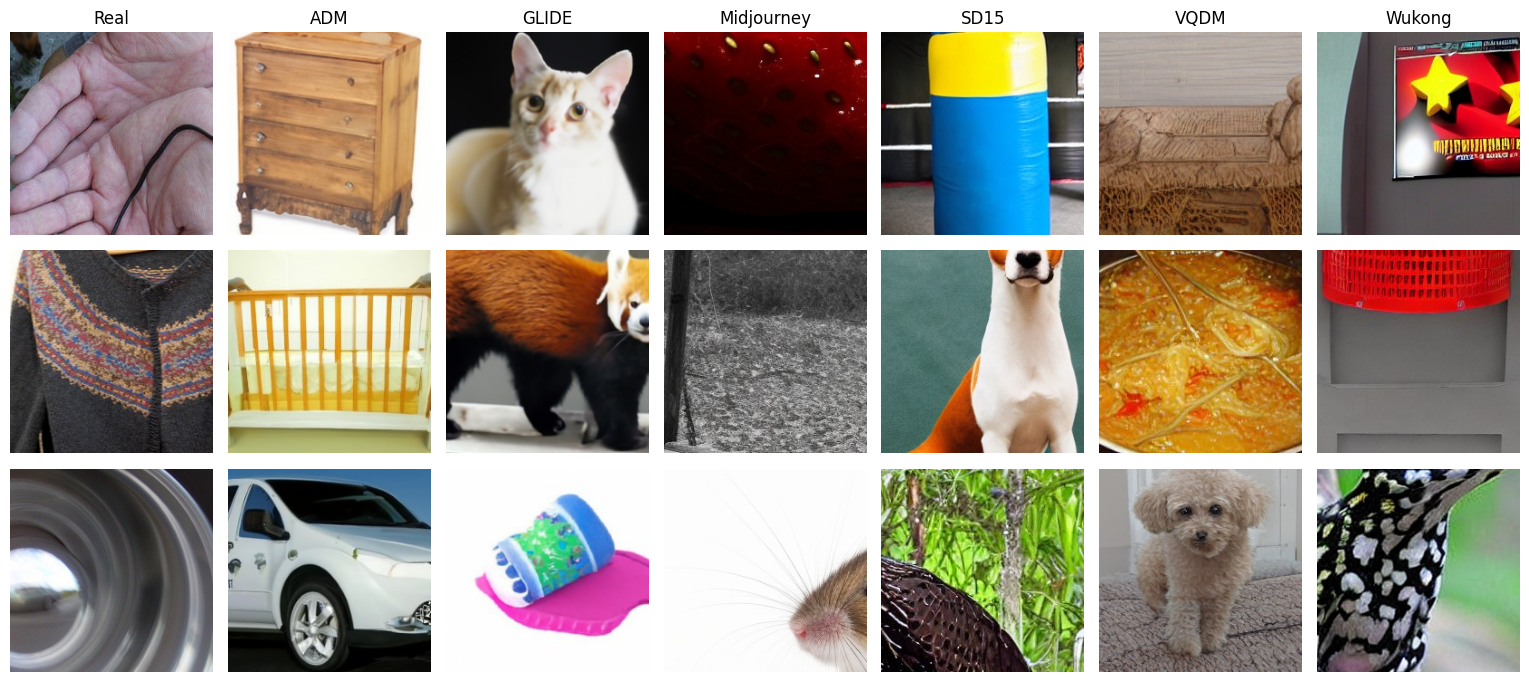
\includegraphics[width=\textwidth]{figures/04_processed_samples.png}
\caption{Processed test images, three per source.}
\label{fig:processed}
\end{figure}

Two limitations remain. First, the generated test images were compressed
with qualities drawn from the training distribution, while the real test
images keep their own, slightly higher, qualities (mean 94.1 versus 92.4).
Second, because generators produce different resolutions, a fixed
$224\times224$ crop covers most of a $256\times256$ ADM image but only a
small region of a $1024\times1024$ Midjourney image
(Figure~\ref{fig:processed}). The apparent zoom level therefore still
varies with the source.

\section{Detection Methods}
\begin{itemize}
  \item \textbf{M1, trained CNN:} a ResNet-50 pre-trained on ImageNet
        and fine-tuned for real-versus-fake classification, following
        the approach of Wang \emph{et al.}~\cite{wang2020cnn}.
  \item \textbf{M2, frozen CLIP features:} image features from a
        pre-trained CLIP model with a linear classifier on top, following
        Ojha \emph{et al.}~\cite{ojha2023universal}.
\end{itemize}

\section{Evaluation Protocol}
% TODO: define metrics (accuracy, AUC, AP, per-class accuracy) when introduced.
Results are reported per generator and per processing condition, not
only as one overall number, and misclassified images are inspected.

% ==================================================================
\chapter{Experimental Setup and Results Analysis}

\section{Setup}
All experiments run on Google Colab with an NVIDIA T4 GPU, using
Python, PyTorch, Pillow, NumPy and pandas. Data and results are stored
on Google Drive.

\section{Pilot Study: File-Level Shortcuts (E0)}
We collected five real photographs (Apple iPhone 17, HEIC) and five
images generated with ChatGPT (PNG). Table~\ref{tab:pilot} shows that
the two classes differ on every file-level property.

\begin{table}[h]
\centering
\small
\begin{tabular}{lll}
\toprule
\textbf{Property} & \textbf{Real (5)} & \textbf{AI-generated (5)}\\
\midrule
Format & HEIF & PNG\\
Resolution (W$\times$H) & $4284\times5712$ & $512\times512$ or $768\times512$\\
File size & 2,404--5,631 KB & 329--524 KB\\
EXIF tags & 11 & 0\\
Embedded colour profile & Yes & No\\
\bottomrule
\end{tabular}
\caption{File properties of the pilot dataset.}
\label{tab:pilot}
\end{table}

A \emph{shortcut rule} labels an image as AI-generated from one file
property, without reading any pixel values. Accuracy is the fraction
of images labelled correctly.

\section{Normalization (E0b)}
Each image was rotated upright using its EXIF orientation, converted to
RGB, center-cropped to $512\times512$ pixels, rebuilt from its raw pixel
array and saved as PNG. A first attempt without the rebuilding step
leaked the iPhone colour profile into all real images, which created a
new shortcut. Table~\ref{tab:shortcuts} compares the rules before and
after normalization.

\begin{table}[h]
\centering
\small
\begin{tabular}{lcc}
\toprule
\textbf{Shortcut rule (predicts ``AI'' if \ldots)} & \textbf{Before (E0)} & \textbf{After (E0b)}\\
\midrule
File format is PNG & 100\% & 50\%\\
Width under 1,000 pixels & 100\% & 50\%\\
File smaller than 1 MB & 100\% & 50\%\\
No EXIF tags & 100\% & 50\%\\
No embedded information & 100\% & 50\%\\
\bottomrule
\end{tabular}
\caption{Accuracy of file-level shortcut rules on the pilot set.}
\label{tab:shortcuts}
\end{table}

\begin{figure}[h]
\centering
\IfFileExists{figures/02_clean_images.png}{%
  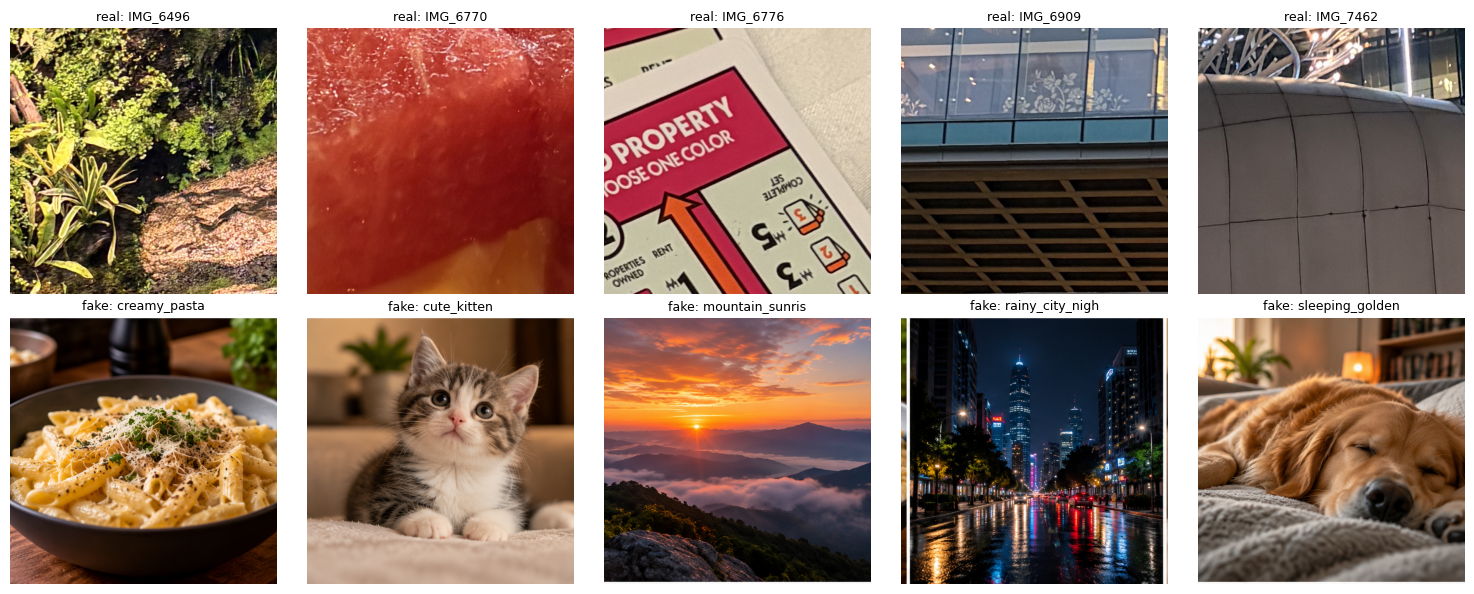
\includegraphics[width=\textwidth]{figures/02_clean_images.png}}{%
  \fbox{\parbox{0.9\textwidth}{\centering Figure placeholder: upload
  \texttt{02\_clean\_images.png} from the results folder to
  \texttt{figures/}.}}}
\caption{Pilot images after normalization. Top: real; bottom: AI-generated.}
\label{fig:pilot}
\end{figure}

Two biases remain that file cleaning cannot remove. Real crops show
close-up textures, while AI images show centred, well-lit whole scenes
(Figure~\ref{fig:pilot}). Real pixels also passed through in-camera
compression, while AI pixels did not.

\section{Real versus AI Detection (E1)}
% TODO
\textit{To be completed.}

\section{Generalization to Unseen Generators (E2)}
% TODO
\textit{To be completed.}

\section{Robustness to Image Processing (E3)}
% TODO
\textit{To be completed.}

\section{Generator Attribution (E4)}
% TODO
\textit{To be completed.}

% ==================================================================
\chapter{Conclusion and Future Work}
% TODO: write after E1--E4.
\textit{To be completed.}

\bibliographystyle{acm}
\bibliography{references}

\end{document}
